\section{Phenomenology of the MSSM}
As the first step towards  phenomenological access to the relevant parameters of the MSSM, we want to have a look at three hypothetically allowed phenomena in the MSSM, that are relatively well controlled by various experimental constraints. For specific regions of the parameter space we encounter that:

\begin{itemize}
	\item The respective lepton numbers $L_{e}$, $L_{\mu}$ and $L_{\tau}$ are not conserved.
	\item Flavor-changing neutral currents (FCNCs) are not suppressed.
	\item New sources of CP-violation are present.
\end{itemize}

\noindent In the MSSM, the non-diagonal terms in the sfermion mass matrices and in the trilinear coupling matrices can induce FCNCs.  In Figure \ref{fig:fcnc} at the beginning of the next page, an hypothetical example process describing such a FCNC is presented. These kind of phenomena are already present in the Standard Model at higher loop orders, but they are highly suppressed which can be explained for example by the GIM-mechanism \cite{GIM1970}, which relates those processes to the unitarity or the presence of complex phases in the CKM matrix. \\
The understanding of CP-violation and its sources in the SM and beyond is very important. In weak interactions CP-violation has extensive implications for the $V$-$A$ structure of the couplings and the non-trivial quark mixing (CKM matrix). Another source of possible CP-violation in the SM is given by the topological $\theta$-term. The famous Sakharov conditions tell us that we need CP-violation in order to describe baryogenesis in the Early Universe. Experimental tests of CP-violation are usually performed in the context of electric dipole moments of electrons and neutrons as well as studies of the Kaon-system. Those measurements put severe constraints on the beforehand presented sources. To give some explicit values we refer for example to \cite{Fischler1992}, where they found out that for TeV-ish sfermion and gaugino masses the absolute values of the complex phases of the gaugino mass parameters, the trilinear couplings and $\abs{\mu}$  have to be $\leq 10^{-2} - 10^{-3}$.\\
\noindent
In the MSSM the amount of new CP-violating phases has increased drastically. This now gives room for two different explanations: One possibility could be that those phases all are approximately zero (which is usually assumed) or there could be non-trivial cancellations amongst the new phases that might lead to tiny measurable effects. In the end this would be a horrible fine tuning task.

\begin{figure}[t]
\centering
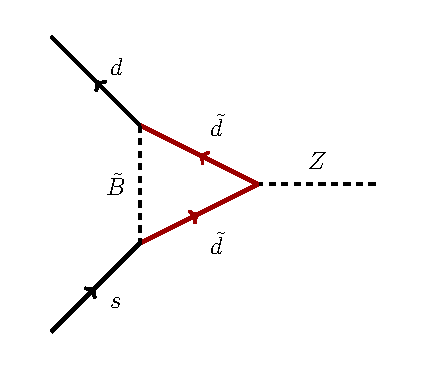
\includegraphics[scale = 0.8]{figures/fcnc_diagram}
\caption{An example diagram for a hypothetical FCNC process ($s \rightarrow d$) in the MSSM involving a Bino and sdown quarks. Such processes can occur if the MSSM squark masses are flavor-violating.}
\label{fig:fcnc}
\end{figure}

\noindent With these general observations at hand we define the \enquote{phenomenological} MSSM (pMSSM) by three basic assumptions \cite{MSSMGroup1998}:

\begin{enumerate}
	\item We do not allow any additional sources of CP-violation. This is implemented by setting all phases in the soft SUSY breaking potential to zero.
	\item We also do not allow processes inducing FCNCs.  This results in a simple, diagonal structure of the sfermion and trilinear coupling matrices.
	\item We assume first and second generation universality, this means we assume that the scalar masses are the same for the first two generations. This is motivated by results on Kaon mixing which put severe constraints on the splitting of the masses. The same we do for the trilinear couplings $A^{u}, A^{d}$ and $A^{\ell}$, usually they are even set to zero since they are not important for phenomenology\footnote{Since they are proportional to the sfermion masses, only the third generation trilinear couplings have phenomenological impact.}.
\end{enumerate}
This already facilitates the general structure of the MSSM a lot! \newpage We summarize the remaining parameters in the pMSSM in the following: 

\begin{itemize}
	\item $\tan\beta = v_u/v_d$, the ratio of the VEVs from the two-Higgs doublets.
	\item $m_{A}^2 = 2m_{12}^2  / \operatorname{sin} 2\beta$, the mass of the pseudoscalar Higgs boson.
	\item $M_{1}$, $M_{2}$ and $M_{3}$, the bino, wino and gluino masses.
	\item $\mu$, the Higgs-higgsino mass parameter.
	\item $m_{\tilde{q}}$, $m_{\tilde{u}_R}$, $m_{\tilde{d}_R}$, $m_{\tilde{\ell}}$ and $m_{\tilde{e}_R}$, the first/second generation sfermion masses.
	\item $m_{\tilde{Q}}$, $m_{\tilde{t}_R}$, $m_{\tilde{b}_R}$, $m_{\tilde{L}}$ and $m_{\tilde{\tau}_R}$, the third generation sfermion masses.
	\item $A^{t}$, $A^{b}$ and $A^{\tau}$, the third generation trilinear couplings.
\end{itemize}
This still leaves 19 open parameters, which makes comprehensive studies of the pMSSM computationally very expensive. In actual experiments we need to construct even more simplified models with only two or three parameters to be able to test any predictions. One possible way to construct such a \enquote{simpler} model, may be to study possible connections to gravity at high energy scales which might render the underlying structure of the theory relatively simple in the high energy regime. This idea is known as mSUGRA und we will present the general concept behind it in the next section. \\
To conclude this section we need to discuss SUSY-breaking. A key problem of the MSSM is, that it fails to give a natural explanation of the fundamental origin of the SUSY breaking parameters. In the last talks we learned about gauge- and gravity mediated SUSY breaking which might provide a way around this problem. We won't go into details here, but for a visualization of the general idea of these concepts, have a look at Figure \ref{fig:susy_breaking}. 
\begin{figure}[H]
\centering
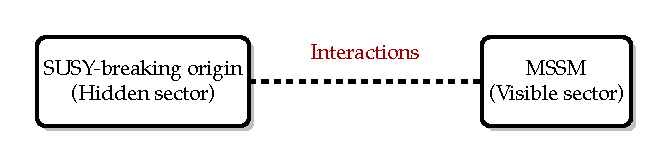
\includegraphics[scale = 1]{figures/susy_breaking}
\caption{Visualization of the idea of gravity-mediated SUSY breaking.}
\label{fig:susy_breaking}
\end{figure}
\noindent
The general idea is that the SUSY-breaking occurs in the hidden sector and is mediated at some messenger scale $M_{\mathrm{mess}}$ via fundamental interactions to the MSSM. The understanding of how SUSY breaking is \enquote{naturally} encoded in this framework might also help to facilitate phenomenological access to the MSSM.